
\section{Numerical Investigations of Antennas in TEM Cells}

\subsection{Preliminary Considerations for Numerical Analysis}

\subsubsection{Skin Effect}

The Skin-effect causes current to flow through a reduced area in a conductor, thus increasing resistance. The imaginary part $\kappa$ of the complex wave number $k$ is described by

\begin{equation}
	\kappa = \omega \sqrt{\frac{\epsilon \mu}{2}}\left[\sqrt{ 1+\left(\frac{\sigma}{\epsilon\omega}\right) ^2 } -1\right]^{1/2}.
	\label{eqn:kappa}
\end{equation}

The skin depth $d$ is responsible for the increased conductor losses and is expressed as 

\begin{equation}
	d = 1/\kappa.
	\label{eqn:skin_depth}
\end{equation}

For highly conductive materials $\left(\sigma \ll \epsilon\omega\right)$ the skin depth is $d \propto 1/\sqrt{\omega}$. Conductor losses $P_\mathrm{loss}$ are linearly proportional to the area of the conductor and therefore Skin-depth. They show the same dependency on the frequency $P_\mathrm{loss}\propto 1/\sqrt{\omega}$ \cite[p. 413]{Griffiths_2024}. Conductor losses contribute to the power consumption of the small loop antenna and is significantly larger than radiation power \cite[p. 231]{Balanis_1997}. 

The investigations in this thesis focus on the coupling behavior of antennas, including the radiation power consumed. All conducting surfaces in the simulation models are perfect electric conductors (PEC) to remove the impact of the Skin-effect.

%reduces the area in which the current flows, therefore increasing resistance. This appears due to the reduction of the depth, in which the electromagnetic waves enter. It is also called Skin depth and mathematically described by \autoref{eqn:skin_depth}. It depends on the imaginary part of the wave number $\kappa$, which is described in \autoref{eqn:kappa}. For high conducting materials $\left(\sigma >> \epsilon\omega\right)$, the dependency of the skin depth $d$ on the frequency can be described therefore as $d \propto 1/\sqrt{\omega}$. Since the power dispersion is linearly proportional to the area of the conductor and therefore Skin-depth, it shows the same dependency on the frequency $P_\mathrm{disp}\propto 1/\sqrt{\omega}$ \cite{Griffiths_2024}.  
%\todo{Own little chapter for skin effect? Loop antennas are known for higher conductor losses than radiation Balanis page 231}
%
%\begin{subequations}
%	\begin{equation}
%		\kappa = \omega \sqrt{\frac{\epsilon \mu}{2}}\left[\sqrt{ 1+\left(\frac{\sigma}{\epsilon\omega}\right) ^2 } -1\right]^{1/2}
%		\label{eqn:kappa}
%	\end{equation}
%	\begin{equation}
%		d = 1/\kappa
%		\label{eqn:skin_depth}
%	\end{equation}
%\end{subequations}
%
%\autoref{fig:deleteafter} shows the total power maintained in the system, meaning $S_{11}^2+S_{12}^2+S_{13}^2$. It does not add up to one, meaning that some energy is lost due to finite conductivity of the septum and antenna. This energy dispersion increases with frequency, most likely due to a decrease of the conductivity due to high-frequency effects like the Skin-effect. Consequently, the power consumption in \autoref{fig:currentlooppowerconsumption} shows a square root relation to the frequency, because the power dispersion is so high. When changing the material of the antenna and septum to a perfect electric conductor, the total power in a system remains one (no power is dispersed) and the power consumption over frequency of the antenna shows a quadratic relation to the frequency, due to the quadratic increase of the radiation resistance.
%
%
%
%At 1\,GHz, the dispersed power already equals to 0.46\,\%, which is much higher than the power transfer of the antenna to one waveport of 1.26e-5 at that frequency. Because this dispersed power is proportional to the square-root of the frequency $P_\mathrm{disp}\propto 1/\sqrt{\omega}$, the overall transferred power to the antenna shows the same characteristic. However, the power transfer to the waveports has a quadratic dependency on the frequency. %This, in turn, also leads to the unusual relation of the electric dipole moment to the frequency. 
%
%This dispersed power may be ignored in the simulations by changing the antenna's material (main source of power dissipation) and the septum from copper to a perfect electric conductor. The overall power in the system then remains at a constant one over the whole frequency range. Additionally, the transferred power to the antenna now has a quadratic relationship with the frequency, indicating increased radiation efficiency, previously described by \autoref{eqn:elec_rad_res}. 
%\todo{Show plots?}

\subsubsection{Antenna models}

Every antenna is fed with a round feedpoint, shown in \autoref{fig:antennaport}. They provide an incident wave of unit power (1\,W). The antenna wires are modeled as PECs with a diameter of 0.2\,mm. The geometry is intentionally kept simple, with the cylindrical wires pointing either in x-, y- or z-direction, without combining multiple orientations. 

\begin{figure}[h]
	\centering
	\includegraphics[width=0.7\linewidth]{content/img/antenna_port}
	\caption{Geometry of an antenna's feedpoint used in simulation. The antenna is fed through a round waveport of diameter $0.46\,\mathrm{mm}$. The antenna consists of PEC wire with diameter of $0.2\,\mathrm{mm}$.	This geometry leads to a reference impedance of $Z_0\approx 50$\,$\Omega$.}
	\label{fig:antennaport}
\end{figure}




\subsubsection{TEM cell model}

The TEM cell model used has a width of $a=40$\,mm, a height of $b=24$\,mm and a length of $l=100$\,mm, shown in \autoref{fig:tem_cell_model}. The cell walls and septum are modeled as PECs. In the TEM cell simulation model, the tapered transition sections at the ports are omitted. This simplification allows unrestricted propagation of higher-order modes, facilitating investigations of their coupling behavior with antennas. \todo{reference section where I discussed this} The reference impedances of the output ports equal $Z_0 \approx 50\,\Omega$.

\begin{figure}[htbp]
	\centering
	\begin{subfigure}[b]{0.48\textwidth}
	\centering
\includegraphics[width=1\linewidth]{content/img/tem_cell_front}
\caption{xy-plane}
\label{fig:temcellfront}
	\end{subfigure}
	\hfill
	\begin{subfigure}[b]{0.48\textwidth}
	\centering
\includegraphics[width=1\linewidth]{content/img/tem_cell_side}
\caption{yz-plane}
\label{fig:temcellside}
	\end{subfigure}
	
	\caption{Geometrical arrangement of the TEM cell used in simulations. The front shows the xy-plane, and the side the yz-plane of the TEM cell.}
	\label{fig:tem_cell_model}
\end{figure}

Upon exciting the output ports, the electric and magnetic energy $W_\mathrm{e}$ and $W_\mathrm{m}$ stored in the TEM cell is derived by \autoref{eqn:em_energy}. The current and voltage at the output ports is found with \crefrange{eqn:iin}{eqn:vin}. The capacitance and inductance of the TEM cell are given by \crefrange{eqn:l_m_energy}{eqn:c_e_energy}. The reactance values fluctuate negligibly over frequency likely due to numerical inaccuracies. The average capacitance and inductance values over the frequency range are chosen. It is assumed that the TEM cell has a constant capacitance and inductance of $C_\mathrm{T} = 6.74\,\mathrm{pF}$ and $L_\mathrm{T} = 16.25\,\mathrm{nH}$. 

\subsubsection{Dipole moments models}\label{sec:prep_dip}

A magnetic dipole moment can be expressed equivalently as either an electric current $I_0$ in a loop, or a magnetic current $I_\mathrm{m}$ in a line, as described in \autoref{eqn:magn_current_curr_loop}. All dipole moments used in the simulations are assumed to be of infinitesimal length, as discussed in \autoref{sec:infinitesimal_electric_dipoles} and \autoref{sec:mag_dip}. For infinitesimal magnetic dipoles, \autoref{eqn:magn_current_curr_loop} simplifies to 

\begin{equation}
	|\mathbf{m}_{\mathrm{m}}|=j\omega\mu_0 |\mathbf{m}_{\mathrm{0}}|,
	\label{eqn:m_mymag_ifa}
\end{equation}

where $\mathbf{m}_{\mathrm{m}}$ with the unit Vm denotes the magnetic dipole moment in the magnetic current representation, and $\mathbf{m}_{\mathrm{0}}$ with the unit Am$^2$ the moment in the electric current representation \cite{10742020}. The simulation models represent magnetic dipole moments with $\mathbf{m}_{\mathrm{m}}$, which will be used in further investigations.

The electric and magnetic dipole moments are placed at the center of the TEM cell at $x=0$, $y=b/2$, $z=0$. As discussed in \autoref{sec:field_dist}, $\mathbf{e}^\pm_\mathrm{TEM}(x=0, y=b/2, z=0)$ has only a y-component at this location, while $\mathbf{h}_\mathrm{TEM}^\pm(x=0, y=b/2, z=0)$ has only an x-component. Consequently, the equivalent dipole moment $\mathbf{m}_{\mathrm{e}}$ is oriented along the y-direction, and $\mathbf{m}_{\mathrm{m}}$ along the x-direction.

Placing $\mathbf{m}_{\mathrm{m}}$ and $\mathbf{m}_{\mathrm{e}}$ in the center of the TEM cell therefore significantly simplifies modeling electrically small antennas with equivalent dipole moments. This assumption is valid for the TEM mode. This configuration is assumed for all numerical investigations following in this thesis, unless otherwise stated.

 When normalizing to the free-space wave impedance $Z_0$, $\mathbf{m}_\mathrm{e}$ can be interchanged with an equivalent $\mathbf{m}_\mathrm{m}$ and vice-versa \cite[p. 414]{Jackson}. Therefore, normalizing either $\mathbf{m}_{\mathrm{e}}$ or $\mathbf{m}_{\mathrm{m}}$ to the free-space wave impedance $Z_0$ enables a meaningful comparison between them.

All simulation results are counterchecked by inserting the equivalent dipole moments into the TEM cell and comparing the power and phase at the output ports with the antenna's results.

\autoref{fig:eyezcouplingcomparison} demonstrates the normalized output power of an electric dipole moment pointing in y-direction, and one in z-direction. This simulation only demonstrates the coupling behavior of the dipole moments over frequency, to explain the non-linear coupling of certain antennas. If dipole moments in certain positions and orientations couple with a different proportionality than the standard two dipole moments (ez and my), then the non-linear coupling may be explained that way.

\begin{figure}[h]
	\centering
	\includegraphics[width=0.5\linewidth]{content/img/ey_ez_coupling_comparison}
	\caption{Comparison of normalized output power of electric dipole moments}
	\label{fig:eyezcouplingcomparison}
\end{figure}



The electric dipole moment in z-direction $e_\mathrm{z}$ demonstrates the expected behavior: As the frequency rises, this dipole moment rises linearly and thus increases the output power quadratically. The electric dipole moment in y-direction $e_\mathrm{y}$ also increases linearly increase with frequency, but does not significantly change the output power for the low frequencies. However, as the frequency approaches the cut-off frequency of the next-higher order mode, the coupling rises significantly.

This simulation is repeated where the dipole moments are located at a height of $h=6\,\mathrm{mm}$, which is the dead center of the TEM cell, and $h=9\,\mathrm{mm}$, which is near the top wall of the TEM cell. The simulation results are similar for both cases. 

Most importantly, this simulation shows that the dipole moments have a relation to the frequency independent on their position. While their magnitude themselves do depend on the position, the relation to the frequency does not. 

An electric dipole in direction of propagation lead to no power transfer, even in higher order modes. That's because these fields do not overlap with the dipole, for which TM modes would be necessary.

\todo{Repeat Simulation for several other dipole moment positions and orientations?} 

As show in the previous simulations, antennas may be represented by dipole moments. This can be done in simulation models, which would otherwise be computationally too effortful. The dipole moments may be put into a shielded enclosure around a larger electronic system, as has been done in \cite{10274360}.

\subsubsection{Mesh modifications}

The mesh determines the resolution of the field quantities over the computational domain. Since electrically small conductors are involved, implementing small mesh elements in their proximity is necessary for accurate modeling of near-fields. Adaptive meshing algorithms may neglect this task, due to the low impact of these near-fields on the solution of the overall computational domain. Consequently, adjusting mesh element sizes does not significantly influence the overall solution of the model, but greatly improves the accuracy of near-field investigations.

The maximum mesh element length in error-prone volumes are adjusted, until the obtained results show a reasonably low amount of numerical artifacts. Such volumes are commonly located adjacent to feedpoints and along edges of small conductors, where large field intensities occur within small spatial regions. The simulation models used in this thesis use roughly 15 elements on the surfaces of such critical volumes to achieve a reasonable representation of these regions while avoiding excessively large meshes.

\subsubsection{S-parameters and derived data}\label{sec:s-param-data}

The TEM cell with an antenna is modeled as a three-port network. The two output ports of the TEM cell are denoted as ports 1 and 2, while the antenna feedpoint is marked as port A. The behavior of this system is fully characterized by its scattering matrix, given as

\begin{equation}
	\left[S\right]=
	\begin{bmatrix}
		S_{11} & S_{12} & S_{1A} \\
		S_{21} & S_{22} & S_{2A} \\
		S_{A1} & S_{A2} & S_{AA}
	\end{bmatrix}.
\end{equation}

The coupling between the antenna and the two ports of the TEM cell are described by S-parameters, specifically the forward transmission coefficients $S_{\mathrm{A1}}$ and $S_{\mathrm{A2}}$. The magnitude of this coefficient is the same for the antenna to both ports $|S_{\mathrm{A1}}|=|S_{\mathrm{A2}}|$, given that the antenna is placed far from the output ports. The power transferred from the antenna $P_{\mathrm{A}}$ to the output ports $P_{\mathrm{1}}$ and $P_{\mathrm{2}}$ is derived through
  
  \begin{equation}
  	P_{\mathrm{A}}=\frac{P_{\mathrm{1}}}{10^{|S_{\mathrm{A1}}|/10}}=\frac{P_{\mathrm{2}}}{10^{|S_{\mathrm{A2}}|/10}}.
  	\label{eqn:power_antenna}
  \end{equation}
  
  Consequently, if the normalized electric field distribution of the TEM mode $\mathbf{e^\pm}_\mathrm{TEM}$ is unknown, it may be derived by setting the output power of a waveport to $P_{\mathrm{1}}=P_{\mathrm{2}}=1/2\,\mathrm{W}$. For example, the uniformly distributed, normalized electric field of the TEM mode along the y-axis at the center of the TEM cell ($z=0$, $x=0$) is derived by
  
  \begin{equation}
  	|a_\mathrm{TEM}|\cdot\mathbf{e}_\mathrm{TEM}^+(x=0,y,z=0)= \frac{\sqrt{P_\mathrm{1}Z_\mathrm{0}}}{b/2}.
  \end{equation}
  
  The difference in phase of $S_{\mathrm{A1}}$ and $S_{\mathrm{A2}}$ influences the magnitude of magnetic dipole moments and electric dipole moments, as discussed in \autoref{sec:equ-dip-mom}. 
%  In this case, a phase shift of $\pi$ indicates the presence of a magnetic dipole moment and the absence of electric dipole moments. This is shown by
%  
%  \begin{subequations}
%  	\begin{equation}
%  		\mathbf{m}_\mathrm{e} = \frac{a+b}{\mathbf{E}^\pm} = \frac{a+a\cdot e^{j\pi}}{\mathbf{E}^\pm} = 0,
%  	\end{equation}
%  	\begin{equation}
%  		\mathbf{m}_\mathrm{m} = j\frac{a-b}{\mathbf{E}^\pm\cdot k_0} = j\frac{a-a\cdot e^{j\pi}}{\mathbf{E}^\pm\cdot k_0} = j\frac{2a}{\mathbf{E}^\pm\cdot k_0}.
%  		\label{eqn:me_phase}
%  	\end{equation}
%  \end{subequations}
%  
%  A phase shift of zero indicates the opposite case. The influence of the electric and magnetic dipole moment is equal, if the phase shift equals $\pi/2$. 
   The peak value of the current through the feedpoint of the antennas is calculated with the S-parameters,
  
  \begin{equation}
  	I_{\mathrm{A}} = \sqrt{2P_{\mathrm{A}}}\frac{(1-S_{\mathrm{AA}})}{\sqrt{Z_0}}.
  	\label{eqn:iin}
  \end{equation}
  
  $P_{\mathrm{A}}$ is the incident power wave applied to the port. 
  The peak voltage at the feedpoint is calculated in a similar fashion as 
 
 \begin{equation}
 	V_{\mathrm{A}} = \sqrt{2P_{\mathrm{A}}}(1-S_{\mathrm{AA}})\sqrt{Z_0}.
 	\label{eqn:vin}
 \end{equation}
 
 Another method to derive voltages and currents is by integration of field intensities. Special care has to be taken at mesh refinement in the area of integration to reduce numerical errors. 
 
 The impedance seen from the antenna feedpoint is 
 
 \begin{equation}
 	Z_{\mathrm{A}}=Z_0\frac{1+S_{\mathrm{AA}}}{1-S_{\mathrm{AA}}}.
 	\label{eqn:za}
 \end{equation}
 
 All values are peak values, unless otherwise stated. 
 
 \subsubsection{Investigation of field regions}
 
\todo[inline]{Update field plots}
 
In this section, the coupling-field regions described in \autoref{sec:rad_fields} are analyzed using the model shown in \autoref{fig:krtemcell}. This analysis examines whether frequency-dependent coupling behavior of the TEM cell can be attributed to changes in the dominant coupling-field region.

 \begin{figure}[h]
 	\centering
 	\includegraphics[width=0.7\linewidth]{content/img/kr_tem_cell}
 	\caption{A TEM cell containing an electric $\mathbf{m}_\mathrm{e}$ and a magnetic dipole moment $\mathbf{m}_\mathrm{m}$ in the center $x=0, y=r=b/4, z=0$ to investigate the field regions in which the coupling occurs.}
 	\label{fig:krtemcell}
 \end{figure} 
 
To determine the influence of the field regions on the coupling effect, $\mathbf{m}_\mathrm{e}$ and  $\mathbf{m}_\mathrm{m}$ are placed in two different TEM cells of dimensions  $a=10\,\mathrm{mm}, b=6\,\mathrm{mm}$ and $a=40\,\mathrm{mm}, b=24\,\mathrm{mm}$. The $k\cdot r$-factor for both cases is shown in \autoref{fig:kranalysissmalltem}.

 \begin{figure}[htbp]
	\centering
	\centering
	\includegraphics[width=0.5\linewidth]{content/img/kr_analysis_small_TEM}
	\caption{$k\cdot r$ in small TEM cell}
	\label{fig:kranalysissmalltem}
	\hfill
\end{figure}

aking the TEM cell smaller such that $k\cdot r \ll 1$, proves to be feasible. The following simulations are conducted with a TEM cell of dimensions $a=10\,\mathrm{mm}$ and $b=6\,\mathrm{mm}$, visible in \autoref{fig:krtemcell}.  
 
 
 First, the current loop antenna used in \autoref{sec:loop_sim} is placed in the dead center of the TEM cell. The equivalent dipole moments are shown in \autoref{fig:loop_small_tem_moments}. In the \autoref{fig:dipole_moments_loop_antenna_copy} next to it, the dipole moments of the same antenna in the larger TEM cell used before ($a=40\,\mathrm{mm}$ and $b=24\,\mathrm{mm}$) are presented. 
 
 \todo[inline]{TODO:Redo plots}
 
 \begin{figure}[htbp]
 	\centering
 	\begin{minipage}[t]{0.48\textwidth}
 		\centering
 		\includegraphics[width=1\linewidth]{content/img/loop_small_tem_moments.png}
 		\caption{Moments in small TEM cell}
 		\label{fig:loop_small_tem_moments}
 	\end{minipage}
 	\hfill
 	\begin{minipage}[t]{0.48\textwidth}
 		\centering
 		\includegraphics[width=1\linewidth]{content/img/dipole_moments_loop_antenna.png}
 		\caption{Moments in normal TEM cell}
 		\label{fig:dipole_moments_loop_antenna_copy}
 	\end{minipage}
 \end{figure}
 
 This is done to compare the dipole moments in both cases. While they clearly increased by magnitude in case of the small TEM cell due to better coupling, their non-linear frequency relation still remains. This means that the change of field regions is not the reason for this behavior.
 
 \todo{TODO: Insert kr, describe where r is measured, describe why the suspicion was that kr could influence this and how the fields change in the regions as described in the theoretical parts. Insert small current loop simulation. Insert Dipole Moment Simulations}
 
 The $k\cdot r$ factor is determined in \autoref{fig:kranalysissmalltem} in the frequency range from 1\,MHz to 3\,GHz for the small TEM cell. This factor does not surpass 0.1, thus fulfilling the requirement $k\cdot r \ll 1$ for this investigation. For comparison, the $k\cdot r$ factor over a wider frequency range are shown in \autoref{fig:kranalysissmalltem} for the normal sized TEM cell ($a = 40\,\mathrm{mm}$ and $b = 24\,\mathrm{mm}$) and a degenerately high TEM cell ($a = 10\,\mathrm{mm}$ and $b=44\,\mathrm{mm}$). The high TEM does not have a port impedance of $50\,\Omega$, and is an attempt to achieve a large $k\cdot r$ factor without higher-order modes propagating. The markers in \autoref{fig:kranalysis} indicate the cut-off frequency, in which the next higher-order mode propagates. They demonstrate, that even in the high TEM cell a $k\cdot r = 1$ is not achieved.
 
 

 \todo[inline]{Fix figures: Titles and Legends. Add kr of normal cell.}
 
% \begin{minipage}[t]{0.48\textwidth}
% 	\centering
% 	\includegraphics[width=1\linewidth]{content/img/kr_analysis}
% 	\caption{$k\cdot r$ for other TEM cells}
% 	\label{fig:kranalysis}
% \end{minipage}
 
 Now, three simulations are conducted with different excitation sources in the small TEM cell:
 
 \begin{itemize}
 	\item The current loop 
 	\item The equivalent dipole sources $e_z$ and $m_m$ of the current loop
 	\item The equivalent magnetic dipole source $m_m$, neglecting $e_z$
 \end{itemize}
 
 \autoref{fig:outputpowercomparisonsmalltem} shows the output power over frequency normalized to 1\,W for all three constellations. The normalization is done to qualitatively discuss the frequency-dependent coupling behavior. \autoref{fig:phaseshiftcomparisonsmalltem} demonstrates the phase shift between the powers at the two waveports over frequency.
 
 \begin{figure}[htbp]
 	\centering
 	\begin{minipage}[t]{0.48\textwidth}
 		\centering
 		\includegraphics[width=1\linewidth]{content/img/output_power_comparison_small_tem}
 		\caption{Output powers}
 		\label{fig:outputpowercomparisonsmalltem}
 	\end{minipage}
 	\hfill
 	\begin{minipage}[t]{0.48\textwidth}
 		\centering
 		\includegraphics[width=1\linewidth]{content/img/phase_shift_comparison_small_tem}
 		\caption{Phase shifts}
 		\label{fig:phaseshiftcomparisonsmalltem}
 	\end{minipage}
 \end{figure}
 
 The frequency dependent behavior of the output power does not change depending on the type of dipole moment used. This is significant, because this shows that the dipole moments do not exhibit different coupling behaviors in the TEM cells. This is further proven in the phase shift plots. The magnetic dipole moment causes a constant phase shift of $-\pi$. If this was not the case, this would mean that the coupling behavior of the magnetic dipole moment in the TEM cell would change. Since the opposite is the case, this poses as good evidence against arguments of change in field regions causing the non-linear dipole moment behavior. Instead, it is very likely to be caused by the geometry of the antenna.

\FloatBarrier
\subsection{Monopole Antenna}\label{sec:monopole}
\subsubsection{Setup}
\FloatBarrier

\begin{figure}[htbp]
	\centering
	\hspace*{-0.0cm}
	\begin{subfigure}[t]{0.48\textwidth}
		\centering
		\includegraphics[height=8cm]{content/img/monopole_near_field}
		\caption{The numerically derived near-field plot of the monopole antenna shows strong displacement currents near the feedpoint and at the wire end. Simulation results are improved by decreasing mesh element lengths in these regions.}
		\label{fig:monopolenearfield}		
	\end{subfigure}
	\hfill
	\begin{subfigure}[t]{0.48\textwidth}
		
		\centering
		\raisebox{0.1cm}{\includegraphics[height=8cm]{content/img/monopole_antenna}}
		\caption{The geometrical aspects of the cylindrical monopole antenna, as implemented in the simulation model.}
		\label{fig:monopoleantenna}
	\end{subfigure}
	
	\caption{}
	\label{fig:field_monopole_antenna}
\end{figure}


The monopole antenna shown in \autoref{fig:monopoleantenna} is installed in the TEM cell and connected to a feed point located on the top wall. The current flowing through it is aligned with the TEM mode and produces an electric dipole moment.

The antenna has a physical length of 5\,mm, making it electrically short for frequencies up to 6,GHz. For frequencies up to 1.25\,GHz, it can be accurately approximated as an infinitesimal electric dipole, as discussed in \autoref{sec:infinitesimal_electric_dipoles}. At higher frequencies, up to 6,GHz, it behaves as a small electric dipole, as explained in \autoref{sec:small_electric_dipole}.




\subsubsection{Equivalent dipole moments}

The corresponding equivalent electric and magnetic dipole moments, $\mathbf{m}_e$ and $\mathbf{m}_m$, are analytically derived using \crefrange{eqn:ifa_me}{eqn:ifa_mm}. The resulting $\mathbf{m}_e$ shown in \autoref{fig:dipolemomentsmonopolewide} increases approximately linearly over frequency, while the magnetic dipole moment is negligible over the whole frequency range. 

Furthermore, the phase difference between the power at the two output ports is zero across the entire frequency range. This observation is consistent with the assumption that a pure electric dipole moment introduces no phase shift between the output port powers, as discussed in \autoref{sec:equ-dip-mom}.


\begin{figure}[htbp]
	\centering
	\includegraphics[width=1\linewidth]{content/img/dipole_moments_monopole_wide}
	\caption{The equivalent electric and magnetic dipole moments analytically calculated with \crefrange{eqn:ifa_me}{eqn:ifa_mm}. To enable direct comparison with the magnetic dipole moment, the electric dipole moment is normalized by the impedance of free space $Z_0$, as discussed in \autoref{sec:prep_dip}.}
	\label{fig:dipolemomentsmonopolewide}
\end{figure}


%\begin{figure}[htbp]
%	\centering
%	\begin{subfigure}[b]{0.48\textwidth}
%		\centering
%		\includegraphics[width=1\linewidth]{content/img/dipole_moments_monopole.png}
%		\caption{Equivalent dipole moments to model the monopole antenna.}
%		\label{fig:dipole_moments_monopole}
%	\end{subfigure}
%	\hfill
%	\begin{subfigure}[b]{0.48\textwidth}
%		\centering
%		\includegraphics[width=1\linewidth]{content/img/phase_shift_monopole}
%		\caption{Phase shift of the power between the output ports produced by the monopole antenna.}
%		\label{fig:phaseshiftmonopole}
%	\end{subfigure}
%	
%	\caption{The equivalent dipole moments and the corresponding induced phase shift of the power between the output ports delivers information about the electric and magnetic coupling behavior of the monopole antenna.}
%	\label{fig:monopole_moments_phase}
%\end{figure}



\subsubsection{Electrical characteristics}

The feedpoint voltage $V$ of the antenna, shown in \autoref{fig:monopolefeedpointvoltagecurrent}, remains largely constant over the investigated frequency range. Consequently, the voltage induced between the antenna and the septum is negligible. This observation is consistent with the absence of a magnetic dipole moment $\mathbf{m}_m$, which is directly related to the induced voltage according to \autoref{eqn:m_v}. 

The feedpoint current $I$, shown in \autoref{fig:monopolefeedpointvoltagecurrent}, increases linearly. The entire current contributes to displacement currents due to the absence of a return path. According to \autoref{eqn:me_i}, $\mathbf{m}_\mathrm{e}$ is proportional to the displacement current to the septum. The linear increase of $\mathbf{m}_\mathrm{e}$ and $I$ are therefore related.

At low frequencies, the antenna impedance in \autoref{fig:monopoleimp} shows a high magnitude, which rapidly decreases as frequency increases. Over the whole frequency range, it exhibits highly capacitive behavior, which is consistent with \autoref{eqn:compl_power_inf_elec_dipole} and the discussion in \autoref{sec:infinitesimal_electric_dipoles}.

\begin{figure}[htbp]
	\centering
	\begin{subfigure}[t]{0.48\textwidth}
		\centering
		\includegraphics[width=1\linewidth]{content/img/monopole_feedpoint_voltage_current}
		\caption{Magnitude of the voltage and current applied at the feedpoint of the monopole antenna over frequency, derived through the S-parameters with \crefrange{eqn:iin}{eqn:vin}.}
		\label{fig:monopolefeedpointvoltagecurrent}
	\end{subfigure}
	\hfill
	\begin{subfigure}[t]{0.48\textwidth}
		\centering
		\includegraphics[width=1\linewidth]{content/img/monopole_imp}
		\caption{Magnitude and phase of the antenna impedance over frequency, derived through the S-parameters with \autoref{eqn:za}.}
		\label{fig:monopoleimp}
	\end{subfigure}
	
	\caption{The electrical characteristics of the monopole antenna over the frequency demonstrate capacitive behavior and a stable feed voltage.}
	\label{fig:monopoleimpvoltcurr}
\end{figure}

%The electric current present in the monopole antenna is aligned with the electric field $\mathbf{e}_\mathrm{TEM}^\pm$ of the dominant TEM mode present in the investigated frequency range. The electric dipole moment in y-direction suffices to model the antenna, because they align with the fields of the TEM mode.

Applying \autoref{eqn:me_i} to determine $\mathbf{m}_\mathrm{e}$ requires knowledge of the magnitude of the displacement current to the septum. Another possibility of determining $\mathbf{m}_\mathrm{e}$ is the integration of the current distribution $I(y)$ weighted by $\mathbf{e}_\mathrm{TEM}^\pm$ along the monopole antenna, as given in \crefrange{eqn:e_int_a}{eqn:e_int_b}. At a frequency of 3,GHz, this approach yields

\begin{equation}
	\mathbf{m}_\mathrm{e}(f=3\,\mathrm{GHz})=\int_{b/2-5\,\mathrm{mm}}^{b/2} I(y, f=3\,\mathrm{GHz})\,dy = 85.69\,\upmu\mathrm{Am}\cdot\mathbf{\hat{a}}_z,
\end{equation}

which corresponds to $\mathbf{m_e}\cdot Z_0=3.23\cdot 10^{-2} \cdot\,\mathrm{Vm}\mathbf\,{\hat{a}}_z$ when normalized by the free-space wave impedance $Z_0$. This approximates $\mathbf{m}_\mathrm{e}$ in \autoref{fig:dipolemomentsmonopolewide} at 3\,GHz reasonably well, therefore supporting \crefrange{eqn:e_int_a}{eqn:e_int_b}. 

%cannot directly be applied using the feedpoint current $I$, since it predominantly gives rise to displacement currents returning to the feedpoint (see \autoref{fig:monopolenearfield}), which do not contribute to the electric coupling.

%According to \autoref{eqn:J1_propagating_waves}, this will lead to a coupling with the output ports. \autoref{eqn:J1_propagating_waves} also requires $\mathbf{e}_\mathrm{TEM}^\pm$ and the part of $I$ contributing to the output power to be in phase at the position of the monopole antenna, due to $\mathbf{e}_\mathrm{TEM}^\pm$ and $\mathbf{h}_\mathrm{TEM}^\pm$ being in-phase at the output ports.

% Using \crefrange{eqn:e_int_a}{eqn:e_int_b} and integrating the current $I$ in \autoref{fig:monopolefeedcurrent} yields





%For example, measuring the y-component of the electric field at the center of output port 1 yields $E_y^+(x=0, y, z=l/2)=15.35\,\mathrm{V/m}$, which is constant over $y$. \todo{differentiate somehow between normalized and normal electric field}. Using the Lorentz Reciprocity theorem \autoref{eqn:J1_propagating_waves}, and integrating $E_y^+(x=0, y, z=l/2)$ and $I(x=0, y, z=l/2)$ over the length of the monopole antenna yields \todo{all values must be peak values}

%\begin{equation}
%	\int_C E_y^+(x=0, y, z=l/2)\cdot I(x=0, y, z=l/2)\,dy=521.9\,\mathrm{\mu W}=2a^2.
%\end{equation}
%
%Applying \autoref{eqn:ifa_me} to then derive the electric dipole moment leads to 
%
%\begin{equation}
%	\mathbf{m}_e = \sqrt{2}\frac{521.9\,\mathrm{W}}{\mathbf{E^\pm}}=
%\end{equation}

The derived equivalent dipole moments $\mathbf{m}_e$, $\mathbf{m}_m$ in the TEM cell produce the output power over frequency shown in \autoref{fig:monopolemomentcomp}, where they are compared with the output power produced by the monopole antenna. The equivalent dipole moment approximation of the monopole antenna loses precision when approaching the cut-off frequency of the first higher-order mode TE\textsubscript{01}. Considering the coefficients $a_{\mathrm{TE}01}$ and $b_{\mathrm{TE}01}$ of the TE\textsubscript{01}-moment increases accuracy, which is not done here.


\begin{figure}[htbp]
	\centering
	\begin{subfigure}[t]{0.48\textwidth}
		\centering
		\includegraphics[width=1\linewidth]{content/img/monopole_output_power}
		\caption{Electric field $E_\mathrm{y}$ and power at one output port, derived with the S-parameters in \autoref{eqn:power_antenna}.}
		\label{fig:monopoleoutputpower}
	\end{subfigure}
	\hfill
	\begin{subfigure}[t]{0.48\textwidth}
		\centering
		\includegraphics[width=1\linewidth]{content/img/monopole_moment_comp}
		\caption{Comparison of output power produced by the monopole antenna and its equivalent dipole moments to demonstrate validity of the model.}
		\label{fig:monopolemomentcomp}
	\end{subfigure}
	
	\caption{}
	\label{fig:monopole_power_comp}
\end{figure}

The distribution of the current along the monopole antenna shown in \autoref{fig:monopole_current_dist} is numerically derived by integrating the magnetic field intensity in a closed loop around the wire using Ampère's law. 

Near the feedpoint at $0\,\mathrm{mm}$ non-linear behavior becomes apparent due to significant displacement currents and numerical artifacts in this region. This causes the current to exhibit a steeper decline with non-physical oscillations. 

The current distribution at $3\,\mathrm{GHz}$ (see \autoref{fig:currentdistributionmonopole}) approximates that of a small electric dipole, as described in \autoref{sec:small_electric_dipole}. It shows an approximately linear decrease towards zero.

The current distribution at $1\,\mathrm{MHz}$, shown in \autoref{fig:currentloopchargedistribution1mhz}, also decreases linearly along the monopole antenna. I can be approximated with an infinitesimal electric dipole, as discussed in \autoref{sec:infinitesimal_electric_dipoles}.

\begin{figure}[htbp]
	\centering
	\begin{minipage}[t]{0.48\textwidth}
		\centering
		\centering
		\includegraphics[width=1\linewidth]{content/img/monopole_current_dist}
		\caption{The current distribution along the monopole antenna at $3\,\mathrm{GHz}$ shows a linear decrease, which is common for a small electric dipole.}
		\label{fig:currentdistributionmonopole}
		\hfill
	\end{minipage}
	\hfill
	\begin{minipage}[t]{0.48\textwidth}
		\centering
		\includegraphics[width=1\linewidth]{content/img/current_loop_charge_distribution_1MHz}
		\caption{The current distribution along the monopole antenna at $1\,\mathrm{MHz}$ shows a large decline near the feedpoint due to increased displacement currents. It then approaches a roughly constant current distribution, which is typical for an approximate infinitely small electric dipole.}
		\label{fig:currentloopchargedistribution1mhz}
	\end{minipage}
	\caption{}
	\label{fig:monopole_current_dist}
\end{figure}


\todo[inline]{TODO: Equivalent circuit for Monopole Antennas}

An equivalent circuit is derived in \autoref{fig:chucircuit}, which is known as Chu equivalent circuit for a short dipole \cite{Hansen_Collin_2013}. 


\begin{figure}[htbp]
	\centering
	\includegraphics[width=0.3\linewidth]{content/img/chu_circuit}
	\caption{The Chu equivalent circuit for a short electric dipole models the monopole antenna's behavior. }
	\label{fig:chucircuit}
\end{figure}

\FloatBarrier
\subsubsection{Current distribution on septum and}
\FloatBarrier

\autoref{fig:monopole_surface_currents} shows the surface current density on the septum induced by the monopole antenna at 3\,GHz. The current reaches both output ports in phase, confirming the absence of a phase shift between the output port powers. 

\begin{figure}[htbp]
	\centering
	\begin{subfigure}[b]{1\textwidth}
		\centering
		\includegraphics[width=1\linewidth]{content/img/monopole_surface_currents.png}
		\caption{Current surface density at 3\,GHz, where mostly the TEM-mode propagates.}
		\label{fig:monopole_surface_currents}
	\end{subfigure}
	
	\vspace{1em} % Add vertical space between subfigures
	
	\begin{subfigure}[b]{1\textwidth}
		\centering
		\includegraphics[width=1\linewidth]{content/img/monopole_surface_currents_te01.png}
		\caption{Current surface density of only the TE\textsubscript{01}-mode at 3.3\,GHz with the TEM mode compensated.}
		\label{fig:monopole_surface_current_te01}
	\end{subfigure}
	
	\caption{Current surface densities at different frequencies, below and above the cut-off frequency of the TE\textsubscript{01}-mode.}
	\label{fig:main}
\end{figure}


\autoref{fig:monopole_surface_current_te01} shows the current density of the septum at 3.3\,GHz, with the TEM-mode compensated at the output ports. Due to the magnetic fields propagating in the z-direction, the current on the septum creates a pattern of swirls. Furthermore, the phase shift of the induced power between the output ports is $\pi$. This results from the magnetic field intensities of the TE\textsubscript{01}-mode being in-phase at the output ports, opposed to the magnetic field intensities of the TEM-mode. 

\todo[inline]{idea: offset in z-direction, show surface current how it gets a pahse shift at waveports, and a magnetic dipole moment appears to be induced}
\todo[inline]{idea: offset in x-direction, showing surface current and explaining the decrease in power transfer (normal E-field distribution)}

%If only the TEM mode propagates, only the y-component of an electric dipole moment and the x-component of a magnetic dipole moment generates output power, assuming they are centrally located ($x=0$, $y=b/4$, $z=0$). This is due to the magnetic field containing only an x-component $\mathbf{h}^\pm = h_x^\pm e^{\pm k_0 z}$, and the electric field only an y-component $\mathbf{e}^\pm = e_y^\pm e^{\pm k_0 z}$ at the center of the TEM cell. \todo{Sketch this situation. Also, $e^{\pm k_0 z}$ indicated that at z=0 the dipole moment is located. Consider this in all sketches}
%An offset of dipole moments or propagation of higher order modes lead to different field components of $\mathbf{h}^\pm$ and $\mathbf{e}^\pm$, and therefore to a change in coupling. These effects are investigated numerically in \autoref{sec:dipole_moments}.


\FloatBarrier
\subsubsection{Electromagnetic energy in the TEM cell}
\FloatBarrier

The monopole antenna generates electromagnetic fields within the TEM cell, resulting in stored electromagnetic energy. The frequency-dependent electric energy is shown in \autoref{eqn:em_energy}. Its quadratic increase correlates with the output power in \autoref{fig:monopoleoutputpower}. The corresponding magnetic energy is several orders of magnitude smaller due to the capacitive behavior of the monopole antenna and is therefore neglected. From the stored electric energy, both the real and imaginary components of the power consumed by the antenna can be determined.

Moreover, the effective inductance and capacitance of the monopole antenna inside the TEM cell can be derived from the magnetic and electric energy expressions given in \crefrange{eqn:l_m_energy}{eqn:c_e_energy}. Using the peak value of the electric energy shown in \autoref{fig:monopoleelecenergy}, the capacitance is estimated to be $C\approx108.55\,\mathrm{fF}$.

\begin{figure}[htbp]
	\centering
	\includegraphics[width=1\linewidth]{content/img/monopole_elec_energy}
	\caption{Electric energy determined by integrating the electric field over the TEM cell volume, using \autoref{eqn:em_energy}. }
	\label{fig:monopoleelecenergy}
\end{figure}

%\begin{figure}[htbp]
%	\centering
%	\begin{subfigure}[b]{0.48\textwidth}
%	\centering
%\includegraphics[width=1\linewidth]{content/img/monopole_magn_energy}
%\caption{Magnetic energy determined with \autoref{eqn:em_energy}}
%\label{fig:monopolemagenergy}
%	\end{subfigure}
%	\hfill
%	\begin{subfigure}[b]{0.48\textwidth}
%	\centering
%\includegraphics[width=1\linewidth]{content/img/monopole_elec_energy}
%\caption{Electric energy determined with \autoref{eqn:em_energy}}
%\label{fig:monopoleelecenergy}
%	\end{subfigure}
%	
%	\caption{Peak electromagnetic energy in the TEM cell generated by the monopole antenna}
%	\label{fig:monopole_em_energy}
%\end{figure}


\FloatBarrier

\subsection{Loop antenna}\label{sec:loop_sim}
\subsubsection{Setup}

\FloatBarrier

\begin{figure}[htbp]
	\centering
	\begin{subfigure}[b]{0.48\textwidth}
		\centering
		\includegraphics[width=1\linewidth]{content/img/loop_near_field}
		\caption{}
		\label{fig:loopnearfield}
	\end{subfigure}
	\hfill
	\begin{subfigure}[b]{0.48\textwidth}
		\centering
		\includegraphics[width=1\linewidth]{content/img/loop_antenna}
		\caption{}
		\label{fig:loopantenna}
	\end{subfigure}
	
	\caption{Geometry of loop antenna inserted into the TEM cell with its magnetic near-field. The return path leads into the conducting surface of the cell.}
	\label{fig:loop_moments_phase}
\end{figure}

A square loop antenna is placed in the center of the TEM cell. Each side has a length of 1.6\,mm, hence it is electrically short for frequencies up to 4.69\,GHz. The square form is preferable to a round antenna in the following numerical simulations, due to more accurate mesh modeling and clearer investigation of the resulting dipole moments. The normal vector of the loop surface points in x-direction. The frequency investigated ranges from 1\,MHz to 3\,GHz, unless otherwise stated, and the input power of the antenna remains at 1\,W.

\FloatBarrier
\subsubsection{Equivalent dipole moments}
\FloatBarrier

\begin{figure}[tb]
	\centering
	\begin{subfigure}[t]{0.48\textwidth}
		\centering
		\includegraphics[width=1\linewidth]{content/img/dipole_moments_loop_antenna.png}
		\caption{Dipole moments}
		\label{fig:dipole_moments_loop_antenna}
	\end{subfigure}
	\hfill
	\begin{subfigure}[t]{0.48\textwidth}
		\centering
		\includegraphics[width=1\linewidth]{content/img/loop_phase}
		\caption{Phase}
		\label{fig:loopphase}
	\end{subfigure}
	
	\caption{Dipole moments and phase shift of loop antenna.}
	\label{fig:loop_moments_phase}
\end{figure}

The dipole moments are plotted in \autoref{fig:dipole_moments_loop_antenna}. The amount of magnetic flux passing through the area of the loop antenna lead to the large magnitude of $\mathbf{m}_m$, as described by \crefrange{eqn:e_a_closed_int}{ eqn:e_b_closed_int} and \autoref{eqn:m_v}. $\mathbf{m}_e$ is created by the current in the loop antenna according to \crefrange{eqn:e_int_a}{ eqn:e_int_b}, which partially points in direction of $\mathbf{e}^\pm_\mathrm{TEM}$. Opposed to the case of a monopole antenna, $\mathbf{m}_e$ and $\mathbf{m}_m$ demonstrate non-linear behavior over frequency, which is investigated further in \autoref{sec:loop_electrical_characteristics}.



\begin{figure}[htbp]
	\centering
	\begin{subfigure}[b]{0.48\textwidth}
		\centering
		\includegraphics[width=1\linewidth]{content/img/loop_opower}
		\caption{}
		\label{fig:loopopower}
	\end{subfigure}
	\hfill
	\begin{subfigure}[b]{0.48\textwidth}
		\centering
		\includegraphics[width=1\linewidth]{content/img/loop_opower_comp}
		\caption{}
		\label{fig:loopopowercomp}
	\end{subfigure}
	
	\caption{Output power of the loop antenna compared with the output power produced by the dipole moments}
	\label{fig:example}
\end{figure}


Possible reasons for the deviation in power are numerical inaccuracies or the coupling of the TE\textsubscript{01} mode.

\FloatBarrier
\subsubsection{Electrical characteristics}\label{sec:loop_electrical_characteristics}
\FloatBarrier

\begin{figure}[htbp]
	\centering
	\begin{subfigure}[b]{0.45\textwidth}
	\centering
\includegraphics[width=1\linewidth]{content/img/loop_elec_energy}
\caption{Electric energy}
\label{fig:loopelecenergy}
	\end{subfigure}
	\hfill
	\begin{subfigure}[b]{0.45\textwidth}
	\centering
\includegraphics[width=1\linewidth]{content/img/loop_mag_energy}
\caption{Magnetic energy}
\label{fig:loopmagenergy}
	\end{subfigure}
	
	\caption{}
	\label{fig:example}
\end{figure}
 
%
%The output power is calculated through the S-parameters. The impedance too. The voltage and current at the antenna port follow from the impedance and input power. The magnetic and electric energy in the TEM cell is calculated through integrating the electric and magnetic field intensities. By dividing them with the voltage and current, the inductance and capacitance of the antenna is calculated.  \todo{Passt so vermutlich nicht: die port s parameter lügen diesbezüglich ein wenig, da sehr viel strom bereits nähe des ports als displacement current zurückfließt.}



\begin{figure}[htbp]
	\centering
	\begin{subfigure}[b]{0.45\textwidth}
	\centering
\includegraphics[width=1\linewidth]{content/img/loop_feed_current}
\caption{Current}
\label{fig:loopfeedcurrent}
	\end{subfigure}
	\hfill
	\begin{subfigure}[b]{0.45\textwidth}
	\centering
\includegraphics[width=1\linewidth]{content/img/loop_feed_voltage}
\caption{Voltage}
\label{fig:loopfeedvoltage}
	\end{subfigure}
	
	\caption{Effective voltage and current at feedpoint of the loop antenna.}
	\label{fig:example}
\end{figure}


The current $I$ in the loop antenna changes along the antenna wire as shown in \autoref{fig:loopfeedreturncurrent}, indicating displacement current coupling to the septum and back to the feedpoint. The difference between the feedpoint and return path current increases over frequency, translating to rising displacement currents. Consequently, $\mathbf{m}_e$ gains a significant magnitude according to \autoref{eqn:me_i}, influencing the electric coupling behavior of the antenna. 

The feedpoint current is derived through integration of $\mathbf{H}$ in a closed loop of radius 0.11\,mm, measured 0.17\,mm above the feedpoint. The return path current is processed with the same loop integration at the same height above the PEC surface. The results vary with height above the PEC surface due to the displacement currents in the near-field.

\begin{figure}[htbp]
	\centering
	\includegraphics[width=0.7\linewidth]{content/img/loop_feed_return_current}
	\caption{Peak currents of loop antenna at feedpoint and return path.}
	\label{fig:loopfeedreturncurrent}
\end{figure}

\todo[inline]{Insert free-space PEC loop simulations.}

\autoref{fig:loopfeedvoltage} demonstrates the voltage at the feedpoint of the antenna, which significantly rises over the frequency. Because the increase in voltage leads to larger displacement current according to \autoref{eqn:me_i}, $\mathbf{m}_e$ follows its frequency-behavior. Similarly, the reduction in current over frequency, shown in \autoref{fig:loopfeedcurrent}, leads a lower induced voltage, and according to \autoref{eqn:m_v} a smaller magnitude of $\mathbf{m}_m$. The current and the voltage are determined with \cref{eqn:vin,eqn:iin}.

\todo[inline]{todo: replace effective voltage and current with peak values for consistency.}

The increases in voltage and decrease in current follows from the impedance, depicted in \autoref{fig:currimp}. The strongly inductive impedance increases linearly over frequency, keeping the input power constant leads to the observed behavior. 

\begin{figure}[htbp]
	\hspace*{4cm}
	\includegraphics[width=0.7\linewidth]{content/img/curr_imp}
	\caption{Magnitude and phase of the impedance of the current loop antenna.}
	\label{fig:currimp}
\end{figure}

\subsubsection{Equivalent circuit model}
A better understanding and an useful model for calculations is an equivalent circuit model. \autoref{fig:eqc_balanis} demonstrates an equivalent circuit for the electrically small loop antenna, where $C$ models stray capacitances, $R_L$ the losses, $R_r$ the radiation, $L_i$ the internal inductance and $L_A$ the external inductance \cite[p. 244] {Balanis_1997}. The model used in the simulation consists of a perfect conductor, therefore $R_L$ and $L_A$ are neglected. Instead, the simplified schematic in \autoref{fig:eqc_simple} is used, where $R_A$, $L_A$ and $C_A$ model the impedance behavior of the antenna.

\begin{figure}[htbp]
	\centering
	\begin{subfigure}[b]{0.45\textwidth}
	\centering
	\resizebox{0.7\textwidth}{!}{
	\begin{tikzpicture}
		% Paths, nodes and wires:
		\draw (11.75, 6) to[european inductor, l={$L_{i}$}] (9.75, 6);
		\draw (12, 2) to[european inductor, l_={$L_{A}$}] (12, 4);
		\draw (7, 6) to[capacitor, l={$C$}] (7, 2);
		\draw (12, 5.75) to[european resistor, l={$R_{r}$}] (12, 3.75);
		\draw (9.25, 6) to[european resistor, l={$R_{L}$}] (7.25, 6);
		\node[ground] at (7, 2){};
		\node[ground] at (12, 2){};
		\draw (7, 6) -- (5, 6);
		\node[circ] at (7, 6){};
		\draw (7, 6) -- (7.25, 6);
		\draw (9.25, 6) -- (10, 6);
		\draw (11.75, 6) -- (12, 6);
		\draw (12, 5.75) -| (12, 6);
		\draw[-latex] (5, 6.5) -- (6.75, 6.5);
		\node[shape=rectangle, minimum width=2.215cm, minimum height=0.965cm] at (6.534, 6.75){} node[anchor=north west, align=left, text width=1.827cm, inner sep=6pt] at (5.409, 7.25){$P_{in}$};
	\end{tikzpicture}
}
\caption{Full equivalent circuit}
\label{fig:eqc_balanis}

	\end{subfigure}
	\hfill
	\hspace*{-0.5cm}
	\begin{subfigure}[b]{0.45\textwidth}
	\centering
	\resizebox{0.65\textwidth}{!}{
	\begin{tikzpicture}
		% Paths, nodes and wires:
		\draw (11, 3) to[european inductor, l_={$L_{A}$}] (11, 5);
		\draw (7, 6) to[capacitor, l={$C_A$}] (7, 2);
		\node[ground] at (7, 2){};
		\node[ground] at (11, 2){};
		\draw (7, 6) -- (5, 6);
		\node[circ] at (7, 6){};
		\draw (7, 6) -- (7.25, 6);
		\draw[-latex] (5, 6.5) -- (6.75, 6.5);
		\node[shape=rectangle, minimum width=2.215cm, minimum height=0.965cm] at (6.534, 6.75){} node[anchor=north west, align=left, text width=1.827cm, inner sep=6pt] at (5.409, 7.25){$P_{in}$};
		\draw (11, 2) -| (11, 3);
		\draw (7.25, 6) to[european resistor, l={$R_A$}] (11, 6);
		\draw (11, 6) -- (11, 5);
	\end{tikzpicture}
}
\caption{Reduced equivalent circuit}
\label{fig:eqc_simple}
	\end{subfigure}
	
	\caption{Equivalent circuits of the small loop antenna.}
	\label{fig:eqc_loop}
\end{figure}


The antenna is placed on a PEC surface in an open space. \todo{sketch}The inductance and capacitance are derived according to \autoref{eqn:m_energy}, in the case of the circuit in \autoref{fig:eqc_simple} this leads to

\begin{subequations}
	\begin{equation}
	L = 2\frac{W_m}{I_{in}^2} = \frac{V_{in}^2}{2\omega^2W_m},
	\end{equation}
 	\begin{equation}
 	C = \frac{2W_c}{V_{in}^2}.
 	\end{equation}
\end{subequations}

\todo[inline]{Plot inductance and capacitance}

In the investigated frequency range, the inductive impedance is significantly smaller than the capacitive impedance, resulting in a predominantly inductive antenna behavior. The model further demonstrates, that the input voltage increases over frequency, therefore increasing the voltage drop across the capacitor. Physically, this corresponds to increased displacement current and electric coupling. 

The result cross-checked with 

\begin{equation}
	L_A = \frac{2\mu_0 l}{\pi} \left[ \ln\!\left(\frac{l}{w_r}\right) - 0.774 \right],
	\label{eqn:ind_approx}
\end{equation}

which is an approximation of the inductance of a square current loop in free-space \cite[p. 245]{Balanis_1997}. There, $l$ is the length of one side of the antenna, and $w_r$ is the wire radius. \autoref{eqn:ind_approx} yields $L=2.32\,\mathrm{nH}$ for the loop antenna in investigation.

The model is extended in \autoref{fig:full_circuit} with an equivalent circuit of the TEM cell, which consists of an equivalent inductance $L_T=L_{T1}+L{T2}$ and capacitance $C_T = C_{T1}+C_{T2}$. After checking the frequency range in which the equivalent circuit of the TEM cell is valid, it is connected with the circuit of the antenna with $C_k$, which models the coupling through displacement current, and the mutual inductances $M_{A,T1}$ and $M_{A,T2}$, which correspond to coupling through induced voltages. The mutual inductances are given as

\begin{equation}
\mathbf{V} = j\omega \begin{bmatrix}
	L_{A} & M_{A,T1} & M_{A,T2} \\
	M_{T1,A} & L_{T1} & 0 \\
	M_{T2,A} & 0 & L_{T2}
\end{bmatrix} \mathbf{I}.
\end{equation}

Due to the modeling of the power transfer with $C_k$, $M_{A,T1}$ and $M_{A,T2}$, the radiation resistance of the antenna shown in \autoref{fig:eqc_simple} is neglected. 

\begin{figure}[htbp]
	\centering
	\resizebox{\textwidth}{!}{%
		\begin{tikzpicture}
			% Paths, nodes and wires:
			\node[shape=circle, draw, line width=1pt, minimum width=0.965cm](N1) at (2.5, 9.5){} node[anchor=east] at (N1.west){$P_\mathrm{in}$};
			\node[ground] at (2.5, 8){};
			\draw (2.5, 9) -| (2.5, 8);
			\draw (4, 11) to[european resistor, l={$R_s$}] (6, 11);
			\draw (7.5, 11) to[capacitor, l={$C_A$}] (7.5, 8);
			\draw (10, 11) to[european inductor, l={$L_A$}] (10, 8);
			\node[ground] at (7.5, 8){};
			\node[ground] at (10, 8){};
			\draw (2.5, 10) -| (2.5, 11) -- (4, 11);
			\draw (6, 11) -- (7.5, 11) -- (10, 11);
			\node[circ] at (7.5, 11){};
			\node[circ] at (10.5, 10){};
			\node[shape=rectangle, draw, line width=1pt, dash pattern={on 4pt off 4pt}, minimum width=4.965cm, minimum height=4.465cm] at (8.5, 9.25){};
			\node[shape=rectangle, minimum width=5.215cm, minimum height=1.465cm] at (8.375, 11.5){} node[anchor=north west, align=left, text width=4.827cm, inner sep=6pt] at (5.75, 12.25){Antenna};
			\draw (10, 11) to[capacitor, l={$C_k$}] (14.5, 11);
			\node[circ] at (10, 11){};
			\draw (14.5, 10) to[european inductor, l={$L_{T2}$}] (18, 10);
			\draw (14.5, 12) to[european inductor, l={$L_{T1}$}] (18, 12);
			\draw (14.5, 10) -| (14.5, 12);
			\node[circ] at (14.5, 11){};
			\draw (18, 10) to[capacitor, l={$C_{T2}$}] (18, 8);
			\draw (23, 10) to[european resistor, l={$R_2$}] (23, 8);
			\node[ground] at (18, 8){};
			\node[ground] at (20.5, 8){};
			\node[circ] at (18, 10){};
			\draw (18, 12) -- (22, 12);
			\draw (20.5, 10) to[capacitor, l={$C_{T1}$}] (20.5, 8);
			\node[ground] at (23, 8){};
			\draw (25.5, 10) to[european resistor, l={$R_1$}] (25.5, 8);
			\node[ground] at (25.5, 8){};
			\draw (22, 12) -- (24.5, 12);
			\draw (20.5, 10) -- (20.5, 12);
			\node[jump crossing] at (20.5, 10){};
			\draw (18, 10) -- (20.36, 10);
			\draw (20.64, 10) -- (23, 10);
			\draw (24.5, 12) -| (25.5, 10);
			\node[circ] at (20.5, 12){};
			\node[shape=rectangle, draw, line width=1pt, dash pattern={on 4pt off 4pt}, minimum width=7.965cm, minimum height=5.715cm] at (18, 9.875){};
			\node[shape=rectangle, minimum width=5.215cm, minimum height=1.465cm] at (16.375, 12.75){} node[anchor=north west, align=left, text width=4.827cm, inner sep=6pt] at (13.75, 13.5){TEM cell};
			\node[shape=rectangle, minimum width=2.715cm, minimum height=0.965cm] at (23.375, 10){} node[anchor=north west, align=left, text width=2.327cm, inner sep=6pt] at (22, 10.5){waveport 2};
			\node[shape=rectangle, minimum width=2.715cm, minimum height=0.965cm] at (26.875, 10){} node[anchor=north west, align=left, text width=2.327cm, inner sep=6pt] at (25.5, 10.5){waveport 1};
			\node[circ] at (15.75, 12.5){};
			\node[circ] at (16.75, 10.5){};
		\end{tikzpicture}
	}
	\caption{Circuit representing the TEM cell, small loop antenna and their coupling.}
	\label{fig:full_circuit}
\end{figure}

%A fine mesh is important due to the near-fields of the antenna. Coarse meshes lead to bad modeling the the fields near the antenna, leading to bad current and voltage calculations in the antenna. A large part of this happens due to bad modeling of the displacement current near the port. Especially small values which are important, such as the capicitance responsible for electric coupling of the antenna, heavily suffer from the numerical error.

%\begin{figure}[htbp]
%	\centering
%	\begin{subfigure}[b]{0.48\textwidth}
%	\centering
%\includegraphics[width=1\linewidth]{content/img/loop_inductance}
%\caption{}
%\label{fig:loopinductance}
%	\end{subfigure}
%	\hfill
%	\begin{subfigure}[b]{0.48\textwidth}
%	\centering
%	\includegraphics[width=1\linewidth]{content/img/loop_capacitance}
%	\caption{}
%	\label{fig:loopcapacitance}
%	\end{subfigure}
%	
%	\caption{Dipole moments and phase shift of loop antenna}
%	\label{fig:example}
%\end{figure}

%The capacitance of the antenna in the TEM cell is $C_{AT}=6.74\,\mathrm{pF}$ and the inductance $L_{AT}=16.51\,\mathrm{nH}$, approximately constant over frequency. In free space, the antenna has much lower inductance and capacitance values, which vary with frequency. \todo{plot free space capacitance and inductance values}

The magnetic dipole moment $\mathbf{m}_m$ is derived by the induced voltage in $L_T1$ and $LT2$ according to \autoref{eqn:m_v}, and the electric dipole moment $\mathbf{m}_e$ by the displacement current in $C_k$ through \autoref{eqn:me_i}. This leads to $\mathbf{m}_e$ and $\mathbf{m}_m$ depicted in \autoref{fig:loopeqcmoments}, which qualitatively agree with the dipole moments of the loop antenna, but deviate in value by up to 15\,\%.

\begin{figure}[htbp]
	\centering
	\includegraphics[width=0.7\linewidth]{content/img/loop_eqc_moments}
	\caption{Equivalent dipole moments derived by the equivalent circuit compared to the dipole moments of the loop antenna in \autoref{fig:dipole_moments_loop_antenna}.}
	\label{fig:loopeqcmoments}
\end{figure}

\FloatBarrier
\subsubsection{Current distribution on septum and higher order modes}
\FloatBarrier

The loop antenna generates a current on the septum of the TEM cell, as shown in \autoref{fig:loop_surface_current}. At a frequency of 3\,GHz, the current arrives at the output ports out of phase, as visible in \autoref{fig:current_loop_surface_current}. This agrees with \autoref{eqn:me_phase}, which predicts a 180\textdegree  phase shift in case of a pure magnetic dipole moment. 

\begin{figure}[htbp]
	\centering
	\begin{subfigure}[b]{1\textwidth}
		\centering
		\includegraphics[width=1\linewidth]{content/img/loop_surface_currents.png}
		\caption{Surface current density of septum induced by loop antenna at 3\,GHz}
	\label{fig:current_loop_surface_current}
	\end{subfigure}
	
	\vspace{1em} % Add vertical space between subfigures
	
	\begin{subfigure}[b]{1\textwidth}
		\centering
		\includegraphics[width=1\linewidth]{content/img/loop_surface_currents_offset_rotation_100MHz}
		\caption{Surface current density of loop antenna with offset of $x=7\,\mathrm{mm}$ and a 90$\textdegree$ rotation angle at 100\,MHz}
		\label{fig:loopsurfacecurrentsoffsetrotation}
	\end{subfigure}
		
	\vspace{1em} % Add vertical space between subfigures
	
	\begin{subfigure}[b]{1\textwidth}
		\centering
		\includegraphics[width=1\linewidth]{content/img/loop_surface_currents_offset_rotation_3GHz3}
		\caption{Surface current density of loop antenna with offset of $x=7\,\mathrm{mm}$ and a 90$\textdegree$ rotation angle at 3.3\,GHz}
		\label{fig:loopsurfacecurrentsoffsetrotation3ghz3}
	\end{subfigure}
	
	\caption{Current surface densities at different frequencies, below and above the cut-off frequency of the TE\textsubscript{01} mode.}
	\label{fig:loop_surface_current}
\end{figure}

\begin{figure}[htbp]
	\centering
	\includegraphics[width=0.7\linewidth]{content/img/loop_surface_currents_offset_rotation_3GHz3_plot}
	\caption{Output power transmitted by the antenna to an output ports through the TEM and TE\textsubscript{01} separately over frequency. TODO: log scale, bigger frequency range}
	\label{fig:loopsurfacecurrentsoffsetrotation3ghz3plot}
\end{figure}

\todo[inline]{TODO: log scale in \autoref{fig:loopsurfacecurrentsoffsetrotation3ghz3plot}. Broader frequency range.}

When the position of the current loop antenna is rotated by 90\textdegree and contains an offset of $x=7\,\mathrm{mm}$, the transmission of power is not possible. As visible in the current distribution \autoref{fig:loopsurfacecurrentsoffsetrotation}, there is no wave propagation and the surface current remains reactive, forming circles around magnetic fields. 

At a frequency of 3.3\,GHz, the TE\textsubscript{01} mode start to propagate, visible in \autoref{fig:loopsurfacecurrentsoffsetrotation3ghz3}. A large proportion of the current now reaches the output ports, providing output power, which is in-phase as opposed to the previous case. The propagation occurs due to the alignment of the current loop with the magnetic field lines in longitudinal direction, which leads to power transfer according to \cref{eqn:e_a_closed_int,eqn:e_b_closed_int}. The output power increases sharply, as demonstrated in \autoref{fig:loopsurfacecurrentsoffsetrotation3ghz3plot}.

\todo[inline]{change jsurf name in legend to surface current}



 
%\autoref{fig:currentloopchargedistribution} shows the charge density distribution in the current loop antenna. Charges collect, among other locations, at the bottom wire. This leads to electric coupling with the septum. 
%
%\begin{figure}[htbp]
%	\centering
%	\begin{minipage}[b]{0.45\textwidth}
%		\centering
%		\includegraphics[width=0.5\linewidth]{content/img/current_loop_charge_distribution}
%		\caption{Charge density distribution in current loop antenna}
%		\label{fig:currentloopchargedistribution}
%	\end{minipage}
%	\hfill
%	\begin{minipage}[b]{0.45\textwidth}
%		\centering
%		\includegraphics[width=0.5\linewidth]{content/img/current_loop_current_distribution}
%		\caption{Current density distribution in current loop antenna}
%		\label{fig:currentloopcurrentdistribution}
%	\end{minipage}
%\end{figure}


%The current and voltage drops along the wire are not constant. From the feedpoint to the first corner, there is a much larger voltage drop and current, than from the second corner to the ground plane. Consequently, the power consumed by the first part is much higher than by the latter \todo{Insert power consumption plots of each antenna section}. Additionally, this difference in power consumption increases slightly over frequency. 

%The electric current reduces over the wire because of the displacement current to the septum and the ground plane. As visible in the charge density plot in \autoref{fig:currentloopcurrentdistribution} and the electric field plot in \autoref{fig:currentloopnearefield}, much of the displacement current occurs near the feedpoint and at the wire parallel to the septum. Consequently, this is where the current drops by the most amount. \todo{Insert current distribution plots}



%\begin{figure}[htbp]
%	\centering
%	\begin{minipage}[b]{0.45\textwidth}
%		\centering
%		\includegraphics[width=0.7\linewidth]{content/img/current_loop_near_e_field}
%		\caption{Electric near field in current loop antenna}
%		\label{fig:currentloopnearefield}
%	\end{minipage}
%	\hfill
%	\begin{minipage}[b]{0.45\textwidth}
%		\centering
%		\includegraphics[width=0.7\linewidth]{content/img/current_loop_near_h_field}
%		\caption{Magnetic near field in current loop antenna}
%		\label{fig:currentloopnearhfield}
%	\end{minipage}
%\end{figure}




%\autoref{fig:currentloopfeedcurrent} and \autoref{fig:currentloopvoltagedrop} show the current and voltage consumption of the antenna. The phase shift equals $\phi\approx89.80\circ$, which hints to a strong inductive behavior. The inductance is determined to be $L\approx2.15\,\mathrm{nH}$. The capacitance is very low, but does lead so some displacement current. The frequency behavior of the voltage and current interchange if the antenna is strongly capacitive, as it the case in a monopole antenna.




%Next, the electric and magnetic near field is investigated. The wave impedance $Z=E/H$ shown in \autoref{fig:waveimpedanceloop} in the center of the loop rises linearly over frequency. At low frequencies, the wave impedance is very low, which confirms the inductive behavior of the antenna. However, as the frequency increases, so does the voltage drop. This may be analogous to a inductor in an electrical circuit, across which the voltage drop also increases with frequency $U = \mathrm{i}L\omega I$. 


%\autoref{eqn:a_b_moments_simp} relates the dipole moments to the output power. The influence of the dipole moments is determined by the electric field at the electric dipole moment and the magnetic field at the magnetic dipole moment. In this formula, the electric and magnetic field are simply related through the free-space wave impedance. However, as visible in \autoref{fig:waveimpedanceloop}, the wave impedance at the location of the dipole moments (i.e. at the antenna) is much lower. Additionally, it rises linearly with the frequency. This influence of the antenna itself on the fields around the dipoles could explain the non-linear relation of the dipole moments to the frequency.



%\autoref{fig:currentlooppowerconsumption} shows the power consumption of the antenna, which is influenced by two factors. The radiation resistance rises quadratically with the frequency. At the same time, the impedance increases, leading to higher matching and therefore to a higher power transfer. This is contrary to the monopole antenna, where the impedance is decreases over the frequency, again leading to better impedance matching, because the impedance was high to begin with. The source impedance is 50\,$\Omega$.



%The current-loop antenna contains two electric dipoles, shifted in phase by 180°. They therefore oppose each other in the power transfer to the waveports. However, as visible in the electric near field plot in \autoref{fig:currentloopvoltagedrop}, the electric dipole moment from node A to the feedpoint is much larger than the one from node B to ground. The reason can be demonstrated by representing the antenna with its nodes in \autoref{fig:current_loop_ua_ub}. The partial inductances in this schematic are much larger than the capacitances. This leads to a large voltage drop between node A and B, and therefore a weaker electric dipole moment at node B.

%Additionally, this voltage difference $V_\mathrm{A}-V_\mathrm{B}$ rises linearly over the frequency, due to the linearly increasing impedance of the inductance $\mathrm{i}\omega L$. This means, that the over electric dipole moment a quadratic relationship to the frequency has.

%Further, \autoref{fig:loopwaveimp} shows the wave impedance of the near-fields at the loop antenna. The \autoref{eqn:a_b_moments_simp} shows, that the influence of the dipoles depends on the electric and magnetic fields at the dipoles position. The electric and magnetic fields are related through the wave impedance $Z = E/H$. If the wave impedance rises linearly over frequency, the electric field increases over the magnetic fields, giving more influence to the electric dipole moments. As previously discussed, there are two electric dipole moments in this antenna, benefiting from that. \todo{Monopole antenna: Also change in wave impedance, but there is not really a magnetic dipole moment} 

%The wave impedance $Z_\mathrm{w}$ in the near field of the electrically small loop antenna is approximated by \autoref{eqn:wave_impedance_loop}. It confirms the linear relationship of the near-field wave impedance to the frequency. \todo{Source: \href{https://en.wikipedia.org/wiki/Near_and_far_field}{Wikipedia}. I couldn't find the source in the reference books. TODO}

%
%\begin{equation}
%	\left|Z_\mathrm{w}\right|\approx 2 \pi^2 \cdot 240\,\Omega \cdot\frac{r\cdot f}{c}
%	\label{eqn:wave_impedance_loop}
%\end{equation}

\FloatBarrier
\subsubsection{Influence of antenna's geometry}
\FloatBarrier

The antenna's geometry influences the coupling behavior. To demonstrate this, the loop antennas presented in are simulated, and their dipole moments and power consumption compared. 

The behavior of the magnetic dipole moments $\mathbf{m}_m$ are equal in all cases according to \crefrange{eqn:e_a_closed_int}{eqn:e_b_closed_int}, since the total area of the loop antenna remains the same. Non-linearities persist, due to almost unchanging capacitance of the antenna to the upper PEC plane, causing increasing displacement current over frequency.

\begin{figure}[htbp]
	\centering
	\begin{subfigure}[t]{0.48\textwidth}
		\centering
		\includegraphics[width=1\linewidth]{content/img/loop-geomg-comp}
		\caption{}
		\label{fig:loop-geomg-comp}
	\end{subfigure}
	\hfill
	\begin{subfigure}[t]{0.48\textwidth}
		\centering
		\includegraphics[width=1\linewidth]{content/img/loop-geom-power}
		\caption{}
		\label{fig:loop-geom-power}
	\end{subfigure}
	
	\caption{Dipole moments and phase shift of loop antenna}
	\label{fig:example}
\end{figure}

The electric dipole moment $\mathbf{m}_e$ is strongly influenced by the antenna's height. An antenna with large $h$ leads to increased displacement currents to the septum.



\FloatBarrier

\subsection{Loop antenna with gap}\label{sec:loop_gap_sim}
\subsubsection{Setup and geometrical analysis}
\FloatBarrier
\begin{figure}[h]
	\centering
	\includegraphics[width=0.5\linewidth]{content/img/gapped_loop_antenna}
	\caption{Geometry of loop antenna with a gap in the return path inserted in the TEM cell.}
	\label{fig:gappedloopantenna}
\end{figure}

The geometry of the loop antenna with a gap is similar to that of the loop antenna discussed in \autoref{sec:loop_sim}. A gap is present with $10\,\upmu\mathrm{m}$ height in the return path, as shown in \autoref{fig:gappedloopantenna}. The magnetic coupling is determined with \crefrange{eqn:e_a_closed_int}{eqn:e_b_closed_int}, leading to 

\begin{equation}
	-\oint_C \boldsymbol{\tau} I(l) \cdot\mathbf{e}_n^\pm  dl= -\int_\text{wire} \boldsymbol{\tau} I_\text{wire}(l) \cdot\mathbf{e}_n^\pm  dl -\int_\text{gap} \boldsymbol{\tau} I_\text{gap}(l) \cdot\mathbf{e}_n^\pm  dl.
\end{equation}

The electric current in the gap is $I_\mathrm{gap}=0\,\mathrm{A}$, while the current in the antenna wire $I_\mathrm{wire}$ is significantly reduced due to the interrupted current path. Consequently, the magnetic coupling between the loop antenna with a gap and the TEM cell is expected to be lower than that of the loop antenna without a gap.

The conductors around the gap act as capacitors, accumulating charges on both sides. This leads to a higher potential in the wire of the antenna. The electric coupling increases significantly, according to \crefrange{eqn:charges_a}{eqn:charges_b}. Concluding, the structure of the loop antenna with the gap suggests capacitive behavior with a dominating electric dipole moment.

\todo[inline]{TODO: Some sources state that electrically small antennas must be either strongly capacitive or inductive. This would mean, that small antennas can always be represented by the same model: Either dominating electric dipole moment in the capacitive antenna case, with a non-linear behavior of the high frequencies, or a magnetic dipole moment with the same property in the inductive antenna case. The frequency, at which the non-linearities occur, depend on the amount of capacitance or inductance, i.e. the Q-factor. A high Q-factor leads to non-linearities in lower cut-off frequencies, and a low Q-factor increases the cut-off frequency. A capacitive antenna with low impedance has a high Q-factor. A inductive antenna with high impedance has a high Q-factor. This can practically be read from the impedance graphs. Can a relation between the impedance/Q-factor and a ``cut-off frequency'' of the dipole moments be established?}

\todo[inline]{TODO: A little thought experiment on the gapped loop antenna demonstrates why this is the case: If the magnetic dipole moment shall be increased in this antenna, the height of the gap can be decreased to increase the current flow and therefore the magnetic coupling. Ironically, this also increases the amount of charges accumulating on the boundaries of the gap, therefore increasing the electric coupling and capacitive behavior. The capacitive behavior can therefore not change, unless the gap is completely removed. Also, the decrease in gap leads to larger total energy transfer and a higher Q-factor. I suspect, that a high Q-factor of an antenna leads to high energy transfer. This would make sense, because a high Q-factor indicates increased near-field intensities, that would naturally couple with the tem cell. A simulation showing the dipole moments for different gap heights over the frequency would support this claim.}

\FloatBarrier
\subsubsection{Equivalent dipole moments}
\FloatBarrier

The electric dipole moment shown in \autoref{fig:gappedloopmoments} clearly dominates over the magnetic dipole moment. The dipole moments behave non-linearly over the frequency. 

\begin{figure}[htbp]
	\centering
	\begin{subfigure}[t]{0.48\textwidth}
		\centering
		\includegraphics[width=1\linewidth]{content/img/gapped_loop_moments}
		\caption{}
		\label{fig:gappedloopmoments}
	\end{subfigure}
	\hfill
	\begin{subfigure}[t]{0.48\textwidth}
	\centering
\includegraphics[width=1\linewidth]{content/img/gapped_loop_phase}
\caption{}
\label{fig:gappedloopphase}
	\end{subfigure}
	
	\caption{Dipole moments and phase shift of loop antenna}
	\label{fig:example}
\end{figure}

\autoref{fig:gappedloopcompmomentsgapsweep} demonstrates the effect of the gap height on the dipole moments' behavior. A larger gap height leads to an decreased charge concentration in the gap region, consequently a smaller magnitude of the electric dipole moment $\mathbf{m}_\mathrm{e}$. Additionally, it also leads to a decrease in electric current $\mathbf{J}$ in the antenna, reducing the magnetic dipole moment $\mathbf{m}_\mathrm{m}$. The reduction in the magnitude of $\mathbf{m}_\mathrm{e}$ and $\mathbf{m}_\mathrm{m}$ with increasing gap height is reflected in the decreasing output power shown in \autoref{fig:gappedloopcomppowergapsweep}.

\begin{figure}[htbp]
	\centering
	\begin{subfigure}[b]{0.48\textwidth}
		\centering
		\includegraphics[width=1\linewidth]{content/img/gapped_loop_comp_moments_gap_sweep}
		\caption{}
		\label{fig:gappedloopcompmomentsgapsweep}
	\end{subfigure}
	\hfill
	\begin{subfigure}[b]{0.48\textwidth}
		\centering
		\includegraphics[width=1\linewidth]{content/img/gapped_loop_comp_power_gap_sweep}
		\caption{}
		\label{fig:gappedloopcomppowergapsweep}
	\end{subfigure}
	
	\caption{Comparison of dipole moments and output power at different gap heights.}
	\label{fig:example}
\end{figure}

An increase in gap height reduces the non-linearities in $\mathbf{m}_\mathrm{e}$ and $\mathbf{m}_\mathrm{m}$. The voltage drop across the gap and the charge accumulation remains stabler over frequency. A small gap leads to both an increase in current and inductance, therefore creating a large voltage drop and influencing $\mathbf{m}_\mathrm{e}$ and $\mathbf{m}_\mathrm{m}$.

\FloatBarrier
\subsubsection{Electrical characteristics}
\FloatBarrier

\begin{figure}[htbp]
	\centering
	\begin{subfigure}[b]{0.48\textwidth}
	\centering
\includegraphics[width=1\linewidth]{content/img/gapped_loop_opower}
\caption{Output electric field and power}
\label{fig:gappedloopopower}
	\end{subfigure}
	\hfill
	\begin{subfigure}[b]{0.48\textwidth}
	\centering
\includegraphics[width=1\linewidth]{content/img/gapped_loop_voltage}
\caption{Peak feed voltage}
\label{fig:gappedloopvoltage}
	\end{subfigure}
	
	\caption{Electric field and power at the TEM cell's output port, and the peak feed voltage of the antenna.}
	\label{fig:example}
\end{figure}



\begin{figure}[htbp]
	\centering
	\begin{subfigure}[b]{0.48\textwidth}
	\centering
\includegraphics[width=1\linewidth]{content/img/gapped_loop_current}
\caption{RMS feed current.}
\label{fig:gappedloopcurrent}
	\end{subfigure}
	\hfill
	\begin{subfigure}[b]{0.48\textwidth}
	\centering
\includegraphics[width=1\linewidth]{content/img/gapped_loop_imp}
\caption{Magnitude and phase of impedance}
\label{fig:gappedloopimp}
	\end{subfigure}
	\label{fig:example}
\end{figure}

The inductance of this antenna is not negligible, opposed to the case of the monopole antenna in \autoref{sec:monopole}. This causes a significant magnitude of $\mathbf{m}_\mathrm{m}$ in \autoref{fig:gappedloopmoments} and a stronger decline in impedance magnitude of the loop antenna with gap, shown in \autoref{fig:gappedloopimp}, compared to the monopole antenna's impedance, demonstrated in \autoref{fig:monopoleimp}.



The gap leads to a significant reduction of electric current. Consequently, the impedance of the antenna shows capacitive behavior, as indicated in \autoref{fig:gappedloopim}. The energy transfer to the TEM cell occurs primarily by displacement current, explaining the dominating electric dipole moment due to \autoref{eqn:me_i}.

\FloatBarrier

\subsection{Inverted-F and center-fed monopole antenna}\label{sec:ifa_sim}

\todo[inline]{TODO}

The inverted-F antenna (IFA) and center-fed monopole antenna are modeled in Ansys HFSS as shown in \crefrange{fig:center_fed_monopole}{fig:ifa}. Both have a maximum dimension of 5\,mm and consequently are electrically small for a frequency of up to 6\,GHz. They are both presented here, because of their similar geometry and electrical behavior. Both posses a current loop with equal area and a bar leading away from it. The bar of the CFM points towards the TEM cell's septum, and the bar of the IFA points towards an output port.

\begin{figure}[htbp]
	\centering
	\begin{subfigure}[c]{0.48\textwidth}
		\centering
		\includegraphics[width=0.6\textwidth]{content/img/center_fed_monopole.png}
		\caption{Center-fed monopole antenna used in simulation}
		\label{fig:center_fed_monopole}
	\end{subfigure}
	\hfill
	\begin{subfigure}[c]{0.48\textwidth}
		\centering
		\includegraphics[width=1\textwidth]{content/img/inverted_f_antenna.png}
		\caption{Inverted F-antenna used in the simulation}
		\label{fig:ifa}
		
		\vspace{1em}
		\centering
		\includegraphics[width=1\linewidth]{content/img/gapped_loop_moments}
		\caption{PLACEHOLDER: Dipole moments comparison}
		\label{fig:gappedloopmoments2}
	\end{subfigure}
	\caption{Main figure caption with one subfigure on the left and two stacked on the right}
	\label{fig:main}
\end{figure}

The center fed monopole antenna is shown in \autoref{fig:center_fed_monopole}. The electric wire with the length of 5 mm points towards the septum. 

\todo[inline]{A question on my mind since the beginning of this thesis: Can how is the magnetic dipole moment influenced by rotating this geometry by 90 degrees? Is the magnetic dipole moment higher or lower than in the rotated loop antenna? With my current knowledge, I suspect that the electric dipole moment leads to current coupling with the TEM cell over displacement current, therefore leading to a smaller magnetic dipole moment then in the case of the loop antenna}

The loop area of the center-fed monopole antenna is equal to that of the loop antenna. Consequently, both antennas exhibit the same magnetic dipole moment.

\todo{CFM at 90° rotation still demonstrates magnetic dipole moment, opposed to current loop. Does this scale with antenna height, i.e. electric dipole moment?}

\FloatBarrier



%\subsubsection{Serial Loop Antenna}
%
%This section will discuss the antenna displayed in \autoref{fig:serialloopantenna}. The idea of that antenna is to create two magnetic dipole moments, which are in phase. As the frequency increases, the displacement current between the loops becomes larger, thus reducing the current through and weakening the second loop. The dipole moments in \autoref{fig:serialloopantennadipolemoments} demonstrate a non-linear behavior of the magnetic dipole moment (only very weakly recognizable, but with a geometry sweep this becomes clearer \todo{Find a geometry where this effect is much stronger}). Also, it would be interesting to measure the wave impedances in both loops over the frequency. Also, find the current distributions, add current plots and electric fields, charge distributions.  
%
%\begin{figure}[h]
%	\centering
%	\includegraphics[width=0.3\linewidth]{content/img/serial_loop_antenna}
%	\caption{Serial loop antenna}
%	\label{fig:serialloopantenna}
%\end{figure}
%\begin{figure}[h]
%	\centering
%	\includegraphics[width=1\linewidth]{content/img/serial_loop_antenna_dipole_moments}
%	\caption{Dipole moments }
%	\label{fig:serialloopantennadipolemoments}
%\end{figure}

\FloatBarrier

